% GNUPLOT: LaTeX picture with Postscript
\begingroup
  \makeatletter
  \providecommand\color[2][]{%
    \GenericError{(gnuplot) \space\space\space\@spaces}{%
      Package color not loaded in conjunction with
      terminal option `colourtext'%
    }{See the gnuplot documentation for explanation.%
    }{Either use 'blacktext' in gnuplot or load the package
      color.sty in LaTeX.}%
    \renewcommand\color[2][]{}%
  }%
  \providecommand\includegraphics[2][]{%
    \GenericError{(gnuplot) \space\space\space\@spaces}{%
      Package graphicx or graphics not loaded%
    }{See the gnuplot documentation for explanation.%
    }{The gnuplot epslatex terminal needs graphicx.sty or graphics.sty.}%
    \renewcommand\includegraphics[2][]{}%
  }%
  \providecommand\rotatebox[2]{#2}%
  \@ifundefined{ifGPcolor}{%
    \newif\ifGPcolor
    \GPcolorfalse
  }{}%
  \@ifundefined{ifGPblacktext}{%
    \newif\ifGPblacktext
    \GPblacktexttrue
  }{}%
  % define a \g@addto@macro without @ in the name:
  \let\gplgaddtomacro\g@addto@macro
  % define empty templates for all commands taking text:
  \gdef\gplbacktext{}%
  \gdef\gplfronttext{}%
  \makeatother
  \ifGPblacktext
    % no textcolor at all
    \def\colorrgb#1{}%
    \def\colorgray#1{}%
  \else
    % gray or color?
    \ifGPcolor
      \def\colorrgb#1{\color[rgb]{#1}}%
      \def\colorgray#1{\color[gray]{#1}}%
      \expandafter\def\csname LTw\endcsname{\color{white}}%
      \expandafter\def\csname LTb\endcsname{\color{black}}%
      \expandafter\def\csname LTa\endcsname{\color{black}}%
      \expandafter\def\csname LT0\endcsname{\color[rgb]{1,0,0}}%
      \expandafter\def\csname LT1\endcsname{\color[rgb]{0,1,0}}%
      \expandafter\def\csname LT2\endcsname{\color[rgb]{0,0,1}}%
      \expandafter\def\csname LT3\endcsname{\color[rgb]{1,0,1}}%
      \expandafter\def\csname LT4\endcsname{\color[rgb]{0,1,1}}%
      \expandafter\def\csname LT5\endcsname{\color[rgb]{1,1,0}}%
      \expandafter\def\csname LT6\endcsname{\color[rgb]{0,0,0}}%
      \expandafter\def\csname LT7\endcsname{\color[rgb]{1,0.3,0}}%
      \expandafter\def\csname LT8\endcsname{\color[rgb]{0.5,0.5,0.5}}%
    \else
      % gray
      \def\colorrgb#1{\color{black}}%
      \def\colorgray#1{\color[gray]{#1}}%
      \expandafter\def\csname LTw\endcsname{\color{white}}%
      \expandafter\def\csname LTb\endcsname{\color{black}}%
      \expandafter\def\csname LTa\endcsname{\color{black}}%
      \expandafter\def\csname LT0\endcsname{\color{black}}%
      \expandafter\def\csname LT1\endcsname{\color{black}}%
      \expandafter\def\csname LT2\endcsname{\color{black}}%
      \expandafter\def\csname LT3\endcsname{\color{black}}%
      \expandafter\def\csname LT4\endcsname{\color{black}}%
      \expandafter\def\csname LT5\endcsname{\color{black}}%
      \expandafter\def\csname LT6\endcsname{\color{black}}%
      \expandafter\def\csname LT7\endcsname{\color{black}}%
      \expandafter\def\csname LT8\endcsname{\color{black}}%
    \fi
  \fi
  \setlength{\unitlength}{0.0500bp}%
  \begin{picture}(7678.00,5280.00)%
    \gplgaddtomacro\gplbacktext{%
      \colorrgb{0.00,0.00,0.00}%
      \put(860,640){\makebox(0,0)[r]{\strut{}0}}%
      \colorrgb{0.00,0.00,0.00}%
      \put(860,1190){\makebox(0,0)[r]{\strut{}0.01}}%
      \colorrgb{0.00,0.00,0.00}%
      \put(860,1740){\makebox(0,0)[r]{\strut{}0.02}}%
      \colorrgb{0.00,0.00,0.00}%
      \put(860,2290){\makebox(0,0)[r]{\strut{}0.03}}%
      \colorrgb{0.00,0.00,0.00}%
      \put(860,2840){\makebox(0,0)[r]{\strut{}0.04}}%
      \colorrgb{0.00,0.00,0.00}%
      \put(860,3389){\makebox(0,0)[r]{\strut{}0.05}}%
      \colorrgb{0.00,0.00,0.00}%
      \put(860,3939){\makebox(0,0)[r]{\strut{}0.06}}%
      \colorrgb{0.00,0.00,0.00}%
      \put(860,4489){\makebox(0,0)[r]{\strut{}0.07}}%
      \colorrgb{0.00,0.00,0.00}%
      \put(860,5039){\makebox(0,0)[r]{\strut{}0.08}}%
      \colorrgb{0.00,0.00,0.00}%
      \put(980,440){\makebox(0,0){\strut{}1.2}}%
      \colorrgb{0.00,0.00,0.00}%
      \put(1772,440){\makebox(0,0){\strut{}1.3}}%
      \colorrgb{0.00,0.00,0.00}%
      \put(2564,440){\makebox(0,0){\strut{}1.4}}%
      \colorrgb{0.00,0.00,0.00}%
      \put(3356,440){\makebox(0,0){\strut{}1.5}}%
      \colorrgb{0.00,0.00,0.00}%
      \put(4149,440){\makebox(0,0){\strut{}1.6}}%
      \colorrgb{0.00,0.00,0.00}%
      \put(4941,440){\makebox(0,0){\strut{}1.7}}%
      \colorrgb{0.00,0.00,0.00}%
      \put(5733,440){\makebox(0,0){\strut{}1.8}}%
      \colorrgb{0.00,0.00,0.00}%
      \put(6525,440){\makebox(0,0){\strut{}1.9}}%
      \colorrgb{0.00,0.00,0.00}%
      \put(7317,440){\makebox(0,0){\strut{}2}}%
      \colorrgb{0.00,0.00,0.00}%
      \put(160,2839){\rotatebox{90}{\makebox(0,0){\strut{}Frecuencia}}}%
      \colorrgb{0.00,0.00,0.00}%
      \put(4148,140){\makebox(0,0){\strut{}Muestra}}%
    }%
    \gplgaddtomacro\gplfronttext{%
      \csname LTb\endcsname%
      \put(6414,4876){\makebox(0,0)[r]{\strut{}Muestra}}%
      \csname LTb\endcsname%
      \put(6414,4676){\makebox(0,0)[r]{\strut{}Distribuci\'on conocida}}%
      \csname LTb\endcsname%
      \put(6414,4476){\makebox(0,0)[r]{\strut{}Newton}}%
      \csname LTb\endcsname%
      \put(6414,4276){\makebox(0,0)[r]{\strut{}Bisecci\'on}}%
    }%
    \gplbacktext
    \put(0,0){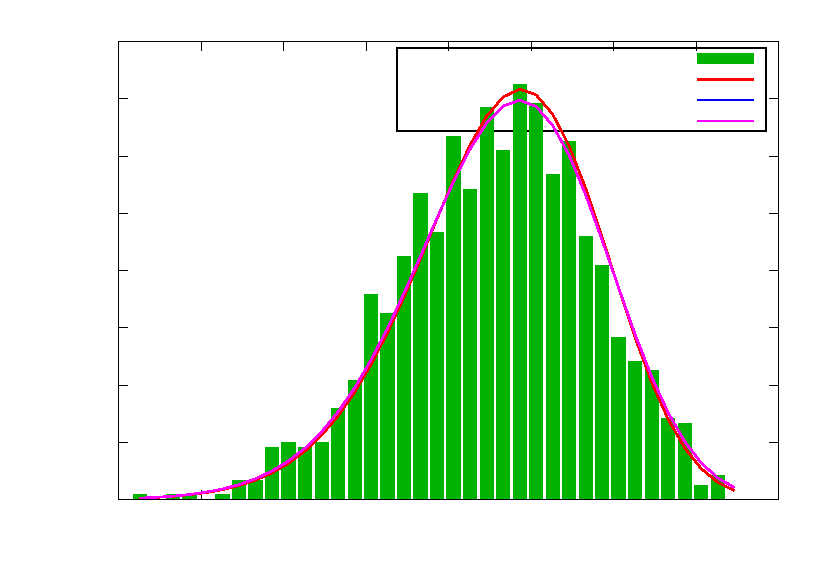
\includegraphics{grafico-distribucion-conocida}}%
    \gplfronttext
  \end{picture}%
\endgroup
